\section{Results: the softmax Ontologizer against SAEs}

\subsection{The price of structure: reconstruction--capacity Pareto}
\label{sec:pareto}

\begin{figure}[tp]\centering
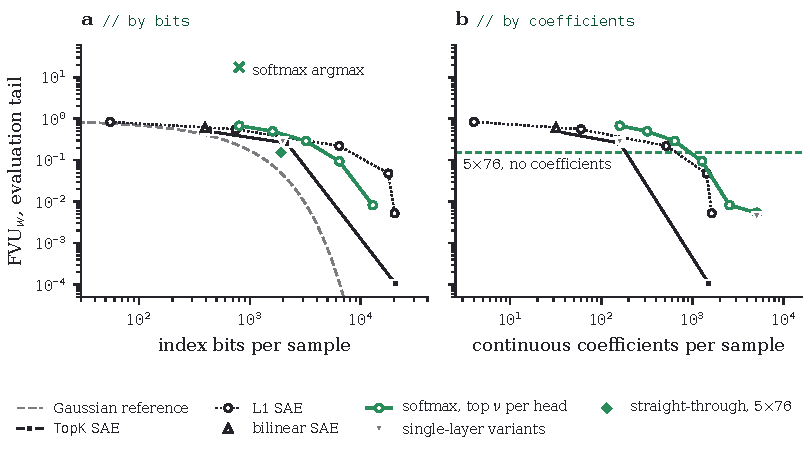
\includegraphics[width=\linewidth]{figures/fig-pareto.pdf}
\caption[Reconstruction against code size]{Reconstruction against code
size on the shared evaluation tail, by index bits (a) and by continuous
coefficients (b): the reference softmax model's truncated codes
(\texttt{resid\_nc}), the SAEs (the L1 SAEs at all five weights of
Table~\ref{tab:cfg-sae}), the single-layer variants and the
straight-through stack (\texttt{ste\_h76\_init01},
Section~\ref{sec:ste}). A code
appears only where its size is nonzero, so the soft codes are in (b)
alone, the softmax argmax is in (a) alone, and the straight-through stack,
whose only continuous numbers are four per-layer gains, is a level in
(b). The dashed curve is the Gaussian reference
(Eq.~\eqref{eq:ratefloor}). Index bits are the whole rate of a hard code,
apart from those gains, but only the support of a code that also sends
coefficients, which is how the $k_{\mathrm{SAE}}{=}32$ and
$k_{\mathrm{SAE}}{=}5120$ SAEs reach the reference in (a);
Figure~\ref{fig:quantrate} puts every code on one rate axis. The softmax
model saw the tail in training and the others hold it out; on rows no
model saw, every point moves by at most 0.3\%, and the dense control's
$1.1\times10^{-4}$ by 0.9\% (Appendix~\ref{app:data}).
One seed per point, except the
$k_{\mathrm{SAE}}{=}32$ SAE's seed-43 replica.}
\label{fig:pareto}
\end{figure}

The SAE frontier dominates the soft Ontologizer's code at every capacity
measured (Figure~\ref{fig:pareto}b). Truncating the reference model's code to the $\nu$ largest
deviations per head from its mean assignment (Appendix~\ref{app:protocols}),
it needs 320 coefficients to reach the $\fvu \approx 0.49$ that the
$k_{\mathrm{SAE}}{=}32$ SAEs reach with 32, and its coarsest code, one
deviation per head (160 coefficients, $\fvu$ 0.677), is already worse than
the SAE's 32-coefficient point, so the very sparse regime is closed to
it. Unstructured reconstruction is better still: the dense control reaches
$\fvu$ $1.1\times10^{-4}$ with $3.4\times$ fewer active coefficients than
the soft code, about $50\times$ lower error at a matched budget. The
truncations are applied after the fact to a model never trained to
truncate, so they may overstate what the structure itself costs: a
residual quantizer degrades when truncated without training for it, and
one trained at a random depth per example does not~\cite{zeghidour2021}. The
code's information is spread across heads: keeping whole heads instead of
deviations is far weaker at matched coefficients ($\fvu$ 0.50 for 8 of 32
heads per layer, against 0.094 at $\nu{=}8$).

The soft model's own discrete reading is not a code. Its argmax
reconstructs at $\fvu$ 17.3, $77\times$ the Gaussian reference for 800
bits (0.226; Figure~\ref{fig:pareto}a), the least distortion an 800-bit code could reach if the
embeddings were Gaussian with their measured covariance
(Eq.~\eqref{eq:ratefloor}). Real embeddings are no harder to compress
than that~\cite[Problem~10.8]{cover2006}, so the argmax sits at least
$77\times$ above the data's distortion--rate function, and on a
selection-sweep run of the same shape the gap is nine orders of magnitude
($8.7\times10^6$ against 0.0007 for the soft code). The entries that
interventions on a softmax model act on are therefore not what carries
its embedding --- the failure VQ-VAE reports for a soft relaxation of
quantization trained from scratch, whose decoder learns to invert the
relaxation~\cite{vandenoord2017} --- which motivates the straight-through
arm of Section~\ref{sec:ste}. The reference does not say that 800 bits are too
few, since non-Gaussian data can be compressed below it.

\subsection{Structure decomposition (the ladder)}

\begin{table}[htbp]\centering\small
\begin{tabular}{@{}lrrl@{}}
\toprule
rung & $\fvu$ & $\mathrm{L0}$ & note \\
\midrule
k32 baseline    & 0.499 & 32   & 0 dead \\
g160top1        & 0.274 & 160  & 1469/5120 dead (29\%) \\
g160softmax     & \textbf{0.0044} & 5120 & beats \texttt{resid\_nc} (0.0054) \\
k32\_p5         & 0.509 & 32   & nested prefixes, $\sim$2\% cost \\
k32\_bl         & 0.602 & 32   & 1920/5120 dead (38\%) \\
\bottomrule
\end{tabular}
\caption{Converged structural rungs, $m{=}5120$, 144.3k steps each.}
\end{table}

Per-head competition sets most of the gap to unstructured codes: the
single-layer soft variant costs about $30\times$ the dense control
($0.0044$ against $1.1\times10^{-4}$). Everything the reference
Ontologizer adds to it (bilinear classifiers, five residual layers, a
shared 2048-dimensional dictionary space) adds nothing to reconstruction,
at $2.2\times$ the parameters. A selection-sweep run of the same shape
does reach 0.0007, six times below the single-layer variant, and keeps
that on rows no model trained on (0.00067 against 0.0044;
Appendix~\ref{app:data}). A stack can therefore beat the single layer out
of sample, but the reference checkpoint does not, so for the model the
rest of this section studies the case has to rest on steering.

Hard per-head selection with a router fused into the classifier
(Appendix~\ref{sec:models}) costs only about 6\% over an unstructured code
of equal sparsity (0.274 for the single-layer hard variant against 0.258
for the $k_{\mathrm{SAE}}{=}160$ SAE). The softmax model's catastrophic
argmax is a training artifact, not a property of discrete head codes:
one-hot selection inflates its output norm $3.7\times$, because winning
atoms carry about $4\times$ the soft mixture's norm, while a stack trained
under the argmax, with no per-head scales at all, reaches $\fvu$ 0.154
(Section~\ref{sec:ste}). A bilinear encoder
costs about 20\% in $\fvu$ and leaves over a third of the dictionary
dead, though its factors start random where every linear rung starts
tied to its decoder (Appendix~\ref{app:configs}), so the cost is not yet
the bilinear form's alone.

Categorical structure appears where it is trained in as hard selection.
The hard variant's partition is head-like, while soft per-head codes
converge to dense, near-uniform mixtures and the SAE's spontaneous groups
are co-firing topical clusters (Appendix~\ref{sec:categorical}). The rest
of the softmax-versus-SAE battery (feature reliability, text fidelity,
language localization and shrinkage) is in Appendix~\ref{app:soft}.

\subsection{Semantic coherence: heads are contrast sets}
\label{sec:prelim-orth}

\begin{figure}[tp]\centering
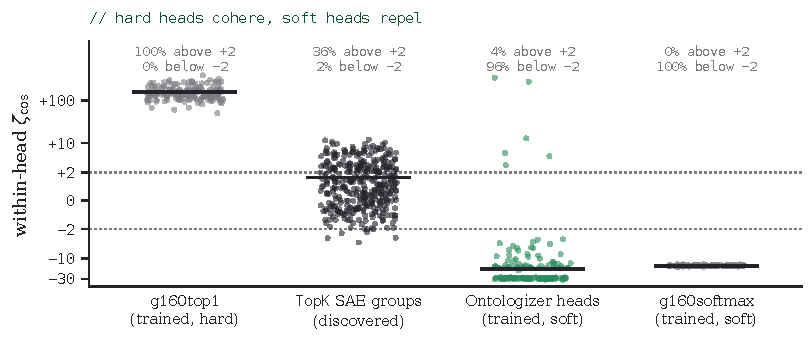
\includegraphics[width=\linewidth]{figures/fig-headcoh.pdf}
\caption[Within-head coherence by head]{Within-head decode-direction
coherence: each head's, or discovered group's, $\zeta_{\cos}$ against a
size-matched null drawn from the same pool ($n_{\mathrm{null}}{=}500$),
on a scale linear between the dotted lines at $\pm2$ and logarithmic
beyond them; bars are means. The
soft heads are those of \texttt{resid\_nc} and \texttt{g160softmax}, the
discovered groups those of the $m{=}11264$, $k_{\mathrm{SAE}}{=}32$ SAE.
One seed per model.}
\label{fig:headcoh}
\end{figure}

Hard-trained heads are coherent, and soft-trained heads are contrast sets
(Figure~\ref{fig:headcoh}).
Every head of the single-layer hard variant decodes to directions far more
similar than a random set of the same size: winner-take-all with a free
magnitude leaves each head one direction at a time, the regime in which
covering a multi-dimensional feature takes many near-collinear
atoms~\cite{dalili2026}, so each head's atoms tile one region. An SAE's post hoc
co-firing groups are mildly coherent, as topical clusters would be. Both
soft architectures show the opposite: in 96--100\% of heads, the entries'
decode directions are more dissimilar than random sets. Softmax
competition pushes a head's atoms apart, so its entries are
well-separated alternatives, and swapping one for another is a large,
clean move along the head's own dimension. The repulsion does not depend
on the inner product: under the whitened metric the objective optimizes,
it strengthens for the Ontologizer (mean $\zeta_{\cos}$ $-24.4$ against
$-17.6$) and is essentially unchanged for the single-layer variants
(Appendix~\ref{sec:coherence}).

The hard-code Ontologizer shows the same in its weights. Its within-head
atom cosine, decoded into output space, is 0.023 at layer 0 and $-0.015$
to $-0.020$ at layers 1--4, so a head's decoded atoms are orthogonal and
slightly repelling; read in the dictionary space instead, the statistic is
dominated by the decoder's null space (Appendix~\ref{sec:rowcos}). Of the
two orthogonalities in Section~\ref{sec:disjoint}, the within-head one
holds in both code types and the between-head one holds in neither: no
trained model partitions its dictionary space between heads. The support
overlap $\omega$ sits at or above a null that shuffles each head's
coordinates, and each head's usage covers 52--98\% of the coordinates,
where a partition into 32 heads needs about 3\%
(Appendix~\ref{sec:support}). Heads are contrast sets that share their
coordinates.

\subsection{Steering fidelity}
\label{sec:steer}

Steering is measured in embedding space: a step from the input along a
direction, scored by whether the target entry becomes selected (its
realization) and by how many other heads change (its collateral, a side
effect inside the code rather than in the downstream features that SAE
steering studies count~\cite{duan2026}; Algorithm~\ref{alg:steerembed}).
The text round trip cannot resolve an
intervention, because even an unsteered round trip preserves a head's
argmax on only 11--13\% of rows (Appendix~\ref{sec:steertext}).

\begin{table}[htbp]\centering\small
\begin{tabular}{@{}lrr@{}}
\toprule
direction & hard code @0.25 / 1.0 & softmax @0.25 / 1.0 \\
\midrule
decode                       & 0.364 / 0.607 & \textbf{0.824} / 0.569 \\
grad                         & 0.304 / 0.103 & 0.453 / 0.477 \\
margin                       & 0.158 / 0.275 & --- \\
adjoint, oriented            & 0.001 / 0.001 & 0.427 / 0.501 \\
adjoint, oriented per sample & ---           & 0.446 / 0.512 \\
random                       & 0.018 / 0.024 & 0.020 / 0.037 \\
\midrule
collateral                   & 0.66 / 0.88   & 0.58 / --- \\
\bottomrule
\end{tabular}
\caption{Realization rate (target entry newly selected) by direction and
strength; 60--64 entries $\times$ 32 held-out rows, chance 0.031.
Collateral agrees within 0.01 across directions at a given strength, so
rows compare at an equal budget. Hard code: the $5\times76$ stack, whose
seed-43 twin agrees within 0.015 in every decode, grad and random
condition. The adjoint direction's orientation is in
Appendix~\ref{sec:eigorient}.}
\label{tab:steerembed}
\end{table}

In embedding space steering works. The decode direction realizes the
target entry on 82\% of rows for the softmax model at strength 0.25. The
hard code is the less steerable of the two: it realizes 36\% while
already disturbing more of the other heads (0.66 against 0.58), because a
hard argmax has margins a small step cannot cross. Swept over strength,
its decode direction saturates near 0.65 (Figure~\ref{fig:steer-curves}b), so a third of its interventions
cannot be realized at any strength, and it passes the soft model only
beyond collateral 0.85, where most of the other heads have moved too.
Steering by target layer reverses the aggregate ranking of the decode and
gradient directions (Appendix~\ref{sec:steerlayer}).

\paragraph{Against supervised steering vectors.} The same measurement
scores the two standard supervised steering vectors for each target: the
difference of means between rows that select the target and rows that do
not (the mean-difference vector of contrastive activation
addition~\cite{rimsky2024}, which averages over many contrast pairs the
single-pair difference of activation addition~\cite{turner2024}), and the
weight vector of a class-balanced logistic probe, both standard supervised
baselines~\cite{wu2025axbenchsteeringllmssimple}, fitted on 8{,}192
reference rows with the steered rows held out. Unlike contrastive
activation addition's pairs, which differ only in the property, these rows
are unpaired, so the difference also carries whatever else varies with
the target. Their labels are the
code's own selections, so they are an oracle baseline: how well a
supervised method that already knew the partition would steer into it.

\begin{table}[htbp]\centering\small
\begin{tabular}{@{}lrrrr@{}}
\toprule
model & own decode & diff.\ of means & probe & random \\
\midrule
softmax stack & \textbf{0.75} / 0.57 & 0.46 / 0.46 & 0.47 / 0.51 & 0.02 / 0.56 \\
hard-code stack & 0.37 / 0.66 & \textbf{0.91} / 0.63 & \textbf{0.94} / 0.64 & 0.02 / 0.65 \\
hard-code flat & 1.00 / 0.33 & 0.97 / 0.27 & 1.00 / 0.31 & 0.01 / 0.37 \\
\texttt{g160top1} & 0.58 / \textbf{0.03} & 0.94 / 0.13 & 0.95 / 0.14 & 0.04 / 0.23 \\
\texttt{g160softmax} & 1.00 / 0.30 & 0.99 / 0.27 & 1.00 / 0.31 & 0.01 / 0.34 \\
$\topk$ SAE, $k_{\mathrm{SAE}}{=}32$ ($m{=}11264$) & 1.00 / 0.21 & 0.92 / 0.21 & 0.97 / 0.23 & 0.00 / 0.25 \\
SAE, bilinear encoder & 1.00 / 0.07 & 0.97 / 0.12 & 0.99 / 0.11 & 0.01 / 0.13 \\
\bottomrule
\end{tabular}
\caption{Each model's own steering direction against supervised vectors
fitted to the same targets (realized / collateral), at a step of
$0.25\lVert \mathbf{x}\rVert$; 64 targets $\times$ 32 held-out rows per
model, one seed. An SAE's collateral counts its other active latents, so
compare within a row.}
\label{tab:steersup}
\end{table}

\begin{figure}[tp]\centering
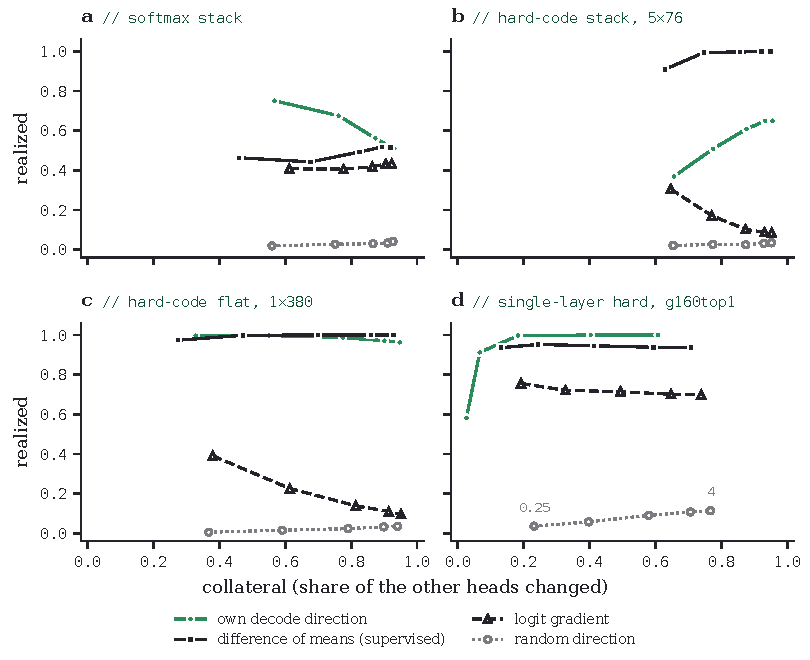
\includegraphics[width=\linewidth]{figures/fig-steer-curves.pdf}
\caption[Steering against collateral by step strength]{Realization
against collateral as the step grows from $0.25\lVert\mathbf{x}\rVert$ to
$4\lVert\mathbf{x}\rVert$, left to right along each curve, on the draw of
Table~\ref{tab:steersup}. (a) The softmax stack
(\texttt{sweep\_softmax\_shm}). (b) The hard-code stack
(\texttt{ste\_h76\_init01}). (c) The flat hard code
(\texttt{ste\_l1\_h380\_i01\_hm1e4}). (d) The single-layer hard variant
\texttt{g160top1}. At each strength the models' own directions disturb
as many other heads as the random step (a direction drawn isotropically
in the embedding's raw coordinates), to within about 0.05, except
\texttt{g160top1}'s decode direction, which disturbs far fewer; what a
direction buys is its height above the random curve. The logistic probe
tracks the difference of means (within 0.03 realized, 0.05 collateral)
and is not drawn.}
\label{fig:steer-curves}
\end{figure}

Only the softmax stack's own direction beats the supervised vectors,
reaching its categories on 75\% of rows against 46--47\%. The hard-code
stack's categories are reachable, but its own direction misses them: the
supervised vectors reach the same entries on 91--94\% of rows, where its
decode direction reaches 37\%. The single-layer hard variant trades reach
for precision (58\% realized against 94\%, at a fifth of the collateral);
every other model's own direction disturbs the other heads as much as a
random step does. Knowing the partition buys the supervised vectors
little precision (the difference of means sits at most 0.1 below random's
collateral), and an SAE's decoder direction is already as good as the
oracle. At each method's own step size the difference of means realizes
more in most models, partly by taking longer steps
(Appendix~\ref{sec:steersupnative}). This tests reaching the model's own
categories; Appendix~\ref{sec:steeroverlay} steers toward an external
concept, language, against supervised vectors fitted to its labels.

A single entry can still steer content: on the reference softmax model,
forcing entry 17 of head 8 in layer 1 reliably yields Burmese decodes of
otherwise preserved content.

\subsection{Description specificity (autointerp)}
\label{sec:autointerp}

Individual SAE latents are about twice as describable as individual
entries. Under the same plain summarization prompt, 51\% of
$k_{\mathrm{SAE}}{=}32$ latents receive a specific description (20\%
naming a language or script), against 23\% of the reference model's
entries (8\%). Blinded detection over the full campaign agrees:

\begin{table}[htbp]\centering\small
\begin{tabular}{@{}lrrrrrrr@{}}
\toprule
model & density & freq & \texttt{params} & \texttt{eig} & \texttt{acts} & \texttt{cacts} & features \\
\midrule
onto (resid\_nc)   & 100\%  & 10.80\% & 0.039 & ---   & 0.473 & 0.392 & 225 \\
k32                & 0.6\%  & 0.61\%  & 0.139 & ---   & 0.645 & 0.603 & 250 \\
k32\_bl            & 0.6\%  & 2.62\%  & 0.136 & 0.034 & 0.578 & 0.470 & 75 \\
g160top1           & 3.1\%  & 5.08\%  & 0.111 & ---   & 0.646 & 0.594 & 150 \\
g160softmax        & 100\%  & 0.00\%  & 0.086 & ---   & 0.449 & 0.364 & 256 \\
k5120 (dense ctrl) & 45.5\% & 17.97\% & 0.010 & ---   & 0.470 & 0.332 & 256 \\
\bottomrule
\end{tabular}
\caption{Mean per-feature detection F1 by description mode
(Appendix~\ref{app:protocols}). The always-match null is about 0.67, and a
generic description that matches every item scores the null, so generic
descriptions inflate toward it. Density is nominal code density; freq is
the firing rate at the $2/k$ threshold. \texttt{k32\_bl}'s pool is only 75
live features; no null control was recorded for this campaign.}
\label{tab:autointerp}
\end{table}

\begin{figure}[tp]\centering
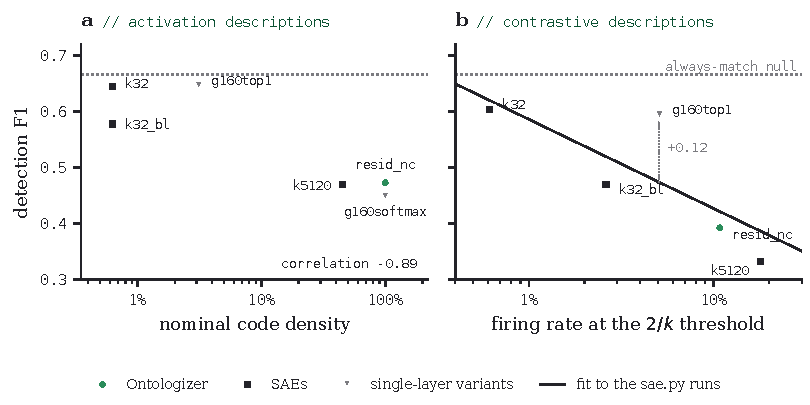
\includegraphics[width=\linewidth]{figures/fig-autointerp-density.pdf}
\caption[Describability against code density]{Mean detection F1 per run
of Table~\ref{tab:autointerp} against code density. (a) Activation
descriptions against nominal density, the share of a code's coefficients
that are nonzero. (b) Contrastive descriptions against the firing rate at
the $2/k$ threshold, with a line fitted in log rate to the four
\texttt{sae.py} runs that fire; \texttt{g160softmax} never crosses the
threshold and is not drawn, and the Ontologizer (\texttt{resid\_nc}) is
held out of the fit. Detection sets are half positives, so a description
that matches every item scores the always-match null, $2/3$ (dotted).
One seed per run.}
\label{fig:autointerp-density}
\end{figure}

Describability tracks code density, not architecture, among the learned
dictionaries compared here (raw model units score lower at similar
sparsity~\cite{paulo2025}). Activation-based
descriptions rank the sparse codes (the $k_{\mathrm{SAE}}{=}32$ SAE and the
single-layer hard variant, 0.65) above the bilinear SAE (0.58), the
reference model and the dense control (0.47) and the single-layer soft
variant (0.45), and density alone carries about 80\% of that variance
(Figure~\ref{fig:autointerp-density}a). The reference Ontologizer sits on
the SAEs' density trend, while the hard variant lies 0.12 above it,
unusually describable for its density (Figure~\ref{fig:autointerp-density}b;
Appendix~\ref{sec:headautointerp}). Per-latent detection F1 therefore
cannot compare architectures at unmatched density, and every soft
Ontologizer is dense by construction. Distribution-based monosemanticity
scores show the same confound, rising as an SAE's L0 falls at fixed
width~\cite{fereidouni2025evaluatingsparseautoencodersmonosemantic}. The contrastive descriptions
(\texttt{cacts}) give the honest number: they score below plain summaries
everywhere, least for the sparse codes (by 0.04--0.05) and most for the
dense control (by 0.14), so part of every plain-summary score is generic
matching.

Parameter-space decodes are not descriptions. Decoding the parameters
scores 0.14 at best (the plain and bilinear SAEs) and 0.04 for the
reference model, where activation descriptions of the same features
score 0.45--0.65. Bilinear eigenfeature decodes score 0.034, but they
decode the top-$|\lambda|$ eigenvector, which for most of the bilinear
SAE's latents is a direction the latent rejects (Appendix~\ref{sec:models}),
so that score does not test eigenfeatures. Part of the parameter decodes'
failure is how the decode is taken: an atom's cosine to its head's mean atom is
0.849, so a raw decode returns one template sentence with the details
shuffled. Subtracting the origin decode makes the decodes legible but not
detectable (on one head, 0.079 against a 0.021 null, where contrastive
activation descriptions score 0.479 against 0.273). A decoded sentence is
an instance of what an entry writes, and detection needs a criterion, so
naming requires activation evidence. Detection also asks an input-side
question of an output-side description; intervention
scoring~\cite{paulo2025} would be the matched test.

\section{A hard-code arm: straight-through selection}
\label{sec:ste}

The softmax model's discrete reading is not its code
(Section~\ref{sec:pareto}), so its argmax entries are not what
interventions act on. Under straight-through selection the forward pass
is the argmax, and no such gap can open: at every checkpoint scored, the
hard and soft-forward reconstructions agree to four decimals.

\subsection{Capacity, and why the head count rises}

A hard code transmits exactly $l\cdot h\log_2 k$ index bits. The Gaussian
reference (Eq.~\eqref{eq:ratefloor}) gives the bits a code would need
to reach a given error if the embeddings were Gaussian; real embeddings
may need fewer:

\begin{center}\small
\begin{tabular}{@{}lrl@{}}
\toprule
$\fvu$ target & bits & heads at $k{=}32$, $l{=}5$ \\
\midrule
0.226 & 800 & 160 (the softmax architecture) \\
0.05 & 1{,}898 & 380 (this arm, $h{=}76$) \\
0.0023 & 4{,}167 & 833 \\
\bottomrule
\end{tabular}
\end{center}

Heads are the cheap axis: bits and parameters both grow linearly in $h$,
and heads run in parallel where layers run in sequence. The arm has
$5\times76$ heads of 32 entries, 1900 bits and 51.93M parameters.
Training a classifier under a hard forward on SONAR takes three settings,
all because the argmax is scale-invariant and, in a naive port, nothing
pushed the logits up from their small initial scale: logit noise relative
to the logit scale, a surrogate temperature matched to that scale, and a
rescaled $s_{\mathrm{KL}_m}$ (Appendix~\ref{sec:calib}; every arm's
configuration is in Table~\ref{tab:cfg-ste-sonar}). The GPT-2 arms ran
without them, at $t{=}1$ with absolute logit noise $\sigma_K{=}0.02$ and
$s_{\mathrm{KL}_m}{=}10^{-6}$ (Table~\ref{tab:cfg-ste-gpt2}), the naive
port's settings, so any comparison between the substrates also compares
two calibrations.

\subsection{Initialization: a third of the error}

The dictionary is non-negative, so a layer's $h$ rows add coherently and
its output grows with $h$. The per-layer gain compounds that, so at the
default initialization the residual grows geometrically with depth: the
first arm started at $1.84\times10^8$ where it should start near 1.
Rescaling each dictionary at initialization so that a layer writes about
a tenth of its input (\texttt{--dict-init-scale 0.1}) divides $h$ out and
starts the cascade as a near-identity:

\begin{table}[htbp]\centering\small
\begin{tabular}{@{}llrrrr@{}}
\toprule
arm & shape & $s_{\mathrm{KL}_m}$ & realized bits & $\fvu$ & params \\
\midrule
\texttt{ste\_h76} (shipped init)    & $5\times76$ & $10^{-4}$ & 1714 (90.2\%) & 0.2293 & 51.93M \\
\texttt{ste\_h76\_init01}            & $5\times76$ & $10^{-4}$ & 1895 (99.7\%) & \textbf{0.1535} & 51.93M \\
\texttt{ste\_h76\_i01\_s43} (seed 43) & $5\times76$ & $10^{-4}$ & 1895 (99.7\%) & \textbf{0.1535} & 51.93M \\
\texttt{ste\_k2\_h380}               & $5\times380$, $k{=}2$ & $5\times10^{-4}$ & 1887 (99.3\%) & 0.1844 & 17.67M \\
\texttt{ste\_l1\_h380\_i01\_hm1e4}   & $1\times380$ & $10^{-4}$ & 1898 (99.9\%) & 0.2750 & 51.93M \\
\texttt{ste\_l1\_h380\_i01}          & $1\times380$ & $5\times10^{-4}$ & 1898 (99.9\%) & 0.2870 & 51.93M \\
\texttt{ste\_l1\_h380\_i01\_s43}     & $1\times380$ & $5\times10^{-4}$ & 1898 (99.9\%) & 0.2871 & 51.93M \\
\bottomrule
\end{tabular}
\caption{Straight-through arms at the fixed initialization (except the
first row), held-out tail. Realized bits are the summed entropy of each
head's argmax usage over the tail, against the nominal $l\,h\log_2 k$; the
sum bounds the information the code carries per sample from above, with
equality only when heads are independent (Eq.~\eqref{eq:realized}).}
\label{tab:init}
\end{table}

One scalar takes a third off the held-out error and has every head using
its entries almost uniformly, the largest single effect in the
straight-through work. It also closes the utilization gap that rescaling
the entropy pressure and whitening the input each closed in part
(Appendix~\ref{sec:calib}). The hard-code results below use the fixed
initialization, except the steering-by-layer and head-health measurements
in Appendix~\ref{sec:steerlayer}.

\paragraph{A discrete code beats $\topk$ SAEs, but not every sparse
code.} On one
frontier of converged SAEs and the single-layer hard variant, all trained
for about 144k steps (Figure~\ref{fig:pareto}a), the stack's 1900 index
bits reach $\fvu$ 0.154. Its only continuous numbers are the gains of
layers 1--4 (layer 0's is identically 1), and with those pinned to their
means it is a pure 1900-bit code at 0.158
(Appendix~\ref{sec:depthdetail}). A code that also sends coefficients
reaches that total only at some precision for them, and no coding of its
coefficients takes an SAE below the least-squares fit on its own support
(Eq.~\eqref{eq:refit}). The $\topk$ SAE with 160 active latents names
them in 1{,}206 bits, so its total is 1900 bits at 4.3 bits per
coefficient, where its error is at least its fit's, 0.236 (0.258 as
trained): at matched total rate the pure code is at least 33\% below
it, and more precise coefficients only lengthen the SAE's code. The
single-layer hard variant, 800 index bits plus 160 coefficients, matches
the rate at 6.9 bits per coefficient, where it is at least 0.273, so the
pure code is at least 42\% below it; it shares the stack's hard per-head
selection but has one layer of linear classifiers and keeps a ReLU
magnitude on each winner. An SAE whose sparsity is not fixed is another
matter. With everything each code sends quantized and entropy-coded
(Appendix~\ref{sec:quantrate}), an L1 SAE with a weak penalty
($s_{\mathrm{L1}}{=}3\times10^{-6}$), quantized coarsely, reaches 0.128 at
1900 bits, 18\% below the stack: its latents fire unevenly, so naming the
active ones costs a fifth less than a fixed-length code would, while the
stack uses its entries almost uniformly and has nothing to save. With
every support charged its fixed-length cost the stack leads every SAE
(0.158 against 0.179). For a hard model the capacity axis is $l\cdot h\log_2 k$ itself:
truncating toward the origin only adds mass the
model was never trained to decode (0.259 at $\nu{=}1$). The stack is less
efficient per bit than a single layer, $3.08\times$ the Gaussian reference
at its rate against $1.28\times$ for one layer's 380-bit prefix, and bits
are not the whole capacity: 380 binary heads, at the same bits, reach
0.1844 (Appendix~\ref{sec:capacity}).

\subsection{Depth at fixed capacity}
\label{sec:depth}

Five layers of 76 heads and one layer of 380 have the same nominal
capacity (1900 bits) and exactly the same parameter count (51.93M; the
dictionary $hke$ and the bilinear classifier $2hkd$ depend on $l$ and $h$
only through $l\cdot h$). At the fixed initialization both use their
entries almost uniformly (summed head entropy 99.7\% and 99.9\% of
nominal), and depth is worth $1.79\times$ the reconstruction error
(0.1535 against 0.2750). Seed does not explain the gap: replicas agree to
four digits. Summed head entropy bounds what each code carries from above,
and whether the two codes carry different amounts jointly is not
measured. Neither arm has converged, and the ratio is narrowing slowly,
but the stack leads at every checkpoint
(Appendix~\ref{sec:depthdetail}).

What depth buys is not usage, input conditioning or the per-layer gain. A
flat arm with a whitened input uses every entry uniformly and still
reconstructs $1.7\times$ worse, and pinning the gains costs the stack only
3.0\% (Appendix~\ref{sec:depthdetail}). Blending each layer's subtracted
reconstruction toward another row's, without retraining, shows instead
that what matters is pairing each residual with its own sample: the error
rises well before the pairing is fully severed. A flat layer decodes like
an additive quantizer~\cite{babenko2014} but does not encode like one:
additive quantization's beam search codes each codebook against what the
codewords already chosen leave, while the layer's heads choose in
parallel, so no head sees another's error --- harmless in a product
quantizer, whose heads own disjoint coordinates, but not when atoms
overlap. The stack is a residual quantizer, each stage coding what earlier
stages missed~\cite{zeghidour2021}. Every stack also trains each of its prefixes
to reconstruct (deep supervision), which a single layer cannot, so
whether the gain needs that supervision or only the residual forward is
not yet separated.

\subsection{Entanglement: the cost of the cascade}
\label{sec:entangle}

A single-head intervention in embedding space realizes its target on
almost every row of the flat model (99.6\%) while disturbing a third of
the other heads; in the stack it realizes 37\% while disturbing 66\%.
Restricting the stack to its layer 0, so that the target is as close to
the input as in the flat model, widens the gap (realized / collateral at
strength 0.25, and at each model's native step for the last row; 12
layer-0 targets in the stack, 64 in the flat arm):

\begin{center}\small
\begin{tabular}{@{}lrr@{}}
\toprule
direction & stack, layer 0 & flat \\
\midrule
decode & 0.049 / 0.680 & \textbf{0.996} / 0.328 \\
grad   & 0.281 / 0.656 & 0.391 / 0.380 \\
margin & 0.034 / 0.661 & 0.076 / 0.379 \\
random & 0.008 / 0.655 & 0.005 / 0.368 \\
\midrule
native decode & 0.044 / 0.678 & 0.169 / 0.043 \\
\bottomrule
\end{tabular}
\end{center}

Collateral is not a property of the intervention. In both models every
direction disturbs as many other heads as a random step of the same
length, to within 0.05 (Figure~\ref{fig:steer-curves}b, c), because the heads sit almost on their decision
boundaries: the median margin between winner and runner-up logits is
$1.5\times10^{-4}$, at layer 0 and in the flat arm alike, so a step of a
quarter of the input's norm crosses many of them. Linearizing each head's
logits with the upstream codes held fixed separates two sources. The
stack's layer-0 heads flip directly about as often as the flat arm's (0.22
against 0.24), so what the stack adds is downstream layers reclassifying a
changed residual: the cascade roughly doubles collateral but is not its
only source. At the model's own step size (the forced entry's output
change, unscaled) the flat arm's step is small (a median 0.028 of
$\lVert\mathbf{x}\rVert$) and moves 4\% of the other heads, while the
stack's (0.13) realizes 8\% of targets across layers and moves 54\%, as a
random step of that length does. This is the steering counterpart of the
composition result, in which non-additivity decays with the number of
layers below an intervention (Section~\ref{sec:formal}). Steering by
target layer, the head-health levers tried against entanglement (only a
row-collinearity setpoint bought steerability), and a head-independence
penalty that turned out to measure estimator bias are in
Appendices~\ref{sec:steerlayer} and~\ref{sec:hsic}.

\subsection{Seed reproducibility: the error is determined, the heads are not}
\label{sec:seeds}

Two runs differing only in seed, both at the fixed initialization, reach
identical held-out error: 0.1535 and 0.1535 for the stack, 0.2870 and
0.2871 for the flat arm (Table~\ref{tab:init}). Nothing that identifies an
individual head agrees:

\begin{center}\small\setlength{\tabcolsep}{4pt}
\begin{tabular}{@{}lrrr@{}}
\toprule
what is compared & stack & flat & null \\
\midrule
head partitions (mean matched NMI) & 0.0121 & 0.0177 & 0.0048 \\
head contributions (centered cosine) & 0.0074 & --- & 0.0015 \\
per-layer subspace, rank 8 & = data's & --- & see text \\
per-head atom Grams & 1.05--1.11$\times$ chance & --- & within-layer pairing \\
\bottomrule
\end{tabular}
\end{center}

Partitions agree barely above the null, where a run scores 0.38 against
its own earlier checkpoint. Contributions agree no better. Per-layer
subspaces agree exactly as much as each model agrees with the data's own
principal directions, and per-head Grams match at chance across seeds,
compared in a canonical entry order that cannot test persistence within a
run (Appendix~\ref{sec:seedsdetail}). What
reproduces is aggregate (the error) or the data's own (its principal
directions), and what identifies an individual head, with one exception,
does not. That is the pattern of weak rather than strong universality, in
which networks trained on the same task share an algorithm while
differing, even between seeds, in the features that
implement it~\cite{chughtai2023}, though equal error alone does not show
that two seeds compute the same reconstruction. Claims about individual heads,
including the Burmese entry and the per-head steering tables, therefore
describe one seed. Non-negativity and the layer-dependent gain put
structure into the floor of every such measure, and several of them,
among them uncentered contributions and subspace overlap, read as
agreement until compared against a null of the same shape.

Layer 0 is the exception in every head-level measure, as the only layer
whose input does not depend on upstream choices, and the one head that
reproduces is there: the topic head of Section~\ref{sec:lang}, the
strongest layer-0 partition in both seeds at different indices, matched
across them at NMI 0.41 against a 0.01 median for other heads. The
softmax Ontologizer fares no better: a seed replica at matched training
matches at most 0.1\% of entries, where the $k_{\mathrm{SAE}}{=}32$ SAE
pair matches 3--31\% (Figure~\ref{fig:softseed}), on a thresholded
activation measure stricter than the decoder-cosine~\cite{song2025positionmechanisticinterpretabilityprioritize}
and activation-correlation~\cite{wang2024} measures on which
language-model SAEs agree across seeds at about 0.8.

\subsubsection{Replication on GPT-2}

A GPT-2 pair differing only in seed ($5\times20$ heads, $k{=}256$,
concatenated heads at $d_{\mathrm{head}}{=}128$, 371{,}900 steps) gives the
same picture. Each measure is run across seeds and, as a positive
control, against the first run's own checkpoint at step 350{,}000
(Figure~\ref{fig:gpt2-seeds}).

\begin{figure}[tp]\centering
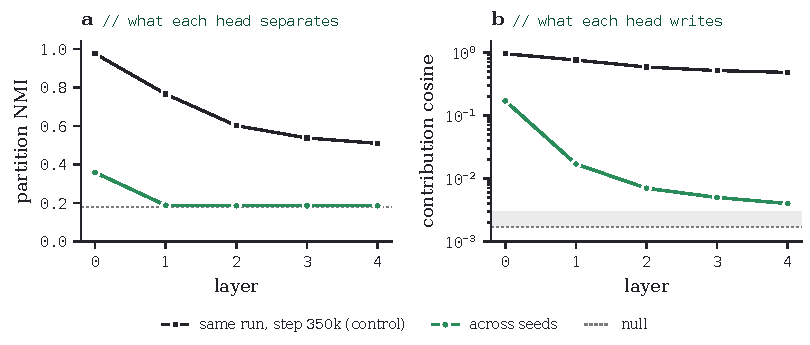
\includegraphics[width=\linewidth]{figures/fig-gpt2-seeds.pdf}
\caption[GPT-2 seed agreement by layer]{The GPT-2 concatenated-head seed
pair by layer: what each head separates (a, partition NMI on 32{,}768
rows) and what it writes (b, centered contribution cosine on 8{,}192
rows, log scale), across the two seeds and against the first run's own
checkpoint at step 350{,}000. Dotted lines are the nulls; the band in (b)
runs from the null's mean to its maximum. One seed pair.}
\label{fig:gpt2-seeds}
\end{figure}

Only layer 0 reproduces, at under a fifth of the control, and each of its
heads matches into the other seed's layer 0 on both measures. Layer 1
keeps its identity (19 and 20 of its 20 heads land in the other seed's
layer 1) while agreeing on almost nothing it separates or writes; layers
2--4 lose even that. The partition null is high, because plug-in NMI
between two 256-way partitions of 32{,}768 rows is dominated by bias, so
it cannot resolve the deep layers; against the tight contribution null
they sit two to four times above it, at about 1\% of the control, which is
real and negligible. The excess over the null is larger than on SONAR
($24\times$ against 5--11$\times$), almost all of it in layer 0, though
the GPT-2 arms also ran without the SONAR arm's calibration
(Table~\ref{tab:cfg-ste-gpt2}; Appendix~\ref{sec:calib}).

\subsubsection{What layer 0's lead is made of}

Three findings, detailed in Appendices~\ref{sec:l0size}
and~\ref{sec:entries}. Layer 0's larger contributions are all gain: it
receives the raw input, while its atoms are no larger than layer 1's
(Table~\ref{tab:gainatoms}), and at equal atom spread it still reproduces
$14\times$ better on GPT-2 and $23\times$ on SONAR. The stack costs
reproducibility at every layer: against flat-arm heads of the same size,
which see the same input with nothing downstream, the stack's layer 0
reproduces about $8\times$ worse and its deeper layers 19--49$\times$
worse, the reproducibility side of entanglement. Within layer 0 the atoms
decide: layer-0 entries are unequal by atom norm rather than usage
(Table~\ref{tab:entries}). On SONAR one head (54) holds 8 of the layer's
11 atoms above three times the median, reproduces at 0.844 against 0.249
for the next, and drives the within-layer correlation between agreement
and largest atom (Table~\ref{tab:bigatoms}); without it the layer-0 mean
falls only from 0.080 to 0.070. GPT-2's layer 0 has no such head: every
head carries a graded tail of large atoms, and agreement is narrowly
spread.

\subsection{Heads against a known factor: language, and what they encode instead}
\label{sec:lang}

Language is the corpus's one factor with free labels, which is why it is
measured, not because a head was expected to encode it: SONAR maps
translations to nearby points~\cite{sonar}, so language is a weak, residual factor of
the embedding. No head encodes it outright. The best reaches a partition
NMI of 0.18 against an attainable 0.875 (0.165 on the second seed), and no
head-health lever changes that (Table~\ref{tab:headlang}). Partitions do
carry the factor well above chance, and the hard code carries more of it:
four times the softmax reference on null-corrected best-head NMI, and 0.42
against 0.28 in a 32-head probe. Single cells and conjunctions of cells
detect language neighborhoods rather than identities (Finnish with
Estonian, Japanese with Korean), which matches an embedding in which
languages are weakly separated regions rather than directions
(Appendix~\ref{sec:langdetail}).

\paragraph{What the strongest head holds: topic and genre.} A semantic,
language-agnostic embedding should be organized by meaning, and its
strongest head is. Ranking layer-0 heads by $\eta^2$ and matching
partitions across runs (65{,}536 held-out rows):

\begin{center}\small\setlength{\tabcolsep}{4pt}
\begin{tabular}{@{}llrrl@{}}
\toprule
run & top head & $\eta^2$ & next head & match across runs \\
\midrule
\texttt{ste\_h76\_init01} (seed 42) & h54 & 0.117 & 0.062 & --- \\
\texttt{ste\_h76\_i01\_s43} (seed 43) & h14 & 0.122 & 0.068 & NMI 0.413 (others 0.010) \\
\texttt{ste\_h76} (unfixed init, seed 42) & h54 & 0.111 & 0.080 & NMI 0.355 (others 0.024) \\
\bottomrule
\end{tabular}
\end{center}

The topic head is the one head found in every run, the strongest
partition in each by nearly a factor of two. A different seed grows it at
a different index, and the same seed keeps its index across the
initialization fix. It is also the head that reproduces on contributions
(Appendix~\ref{sec:entries}), the exception to Section~\ref{sec:seeds}'s
finding that heads do not reproduce, though at NMI 0.41 against a 0.87
same-run control it is the same variable carved differently, not the same
partition. It also carries more language than almost any other head: in
seed 43 it is the most language-informative of all 380 heads (NMI 0.165,
Table~\ref{tab:headlang}) and in seed 42 the third (0.161), though
against an attainable 0.875 each of its entries still mixes many
languages. Decoded as deviations
from the head's mean atom, its entries read as topic and genre: crime
news, geopolitics and parliament, encyclopedic place description,
manufacturing, marketing, legislative text and entertainment. Contrastive
autointerp agrees, with every category of description above its
null (Appendix~\ref{sec:langdetail}). Testing whether heads are natural
variables therefore needs topic or genre labels, which this corpus does
not have.

\section{Hard codes on GPT-2 small: atoms in activation space}
\label{sec:gpt2hard}

A second line of straight-through runs, from the \texttt{headline}
branch, takes the hard code to GPT-2 small and adds what an embedding
substrate lacks: the fraction of GPT-2's loss recovered when the
reconstruction is spliced back into the model,
$(\mathrm{CE}_{\mathrm{ablate}} - \mathrm{CE}_{\mathrm{recon}})
/(\mathrm{CE}_{\mathrm{ablate}} - \mathrm{CE}_{\mathrm{clean}})$, with the
residual mean-ablated as the floor --- a lenient scale against an
ablation floor~\cite{gao2024}, so Table~\ref{tab:gpt2hard}'s caption also
gives the cross-entropies themselves. These runs model the residual stream
entering block 8, one block earlier than the GPT-2 runs of
Section~\ref{sec:seeds}, centered and scaled to unit mean square, on
FineWeb, and their $\fvu$ is unwhitened; they compare only with each other
and with SAEs trained on the same cache. Held-out evaluation uses
documents disjoint from training (520k tokens for the 40M-token runs, 65k
for one-epoch runs).

\paragraph{The design.} Relative to Section~\ref{sec:ste}, three things
change. Atoms are direct: signed vectors in activation space, with no
latent dictionary space and no decoder, so every atom is literally a
steering direction. Every layer, layer 0 included, classifies the unit
direction of what it corrects, and each layer's contribution is scaled by
the observed residual norm, clipped at $\lVert\mathbf{x}\rVert$, which
makes the model positively homogeneous ($f(\xi\mathbf{x}) = \xi
f(\mathbf{x})$ for $\xi > 0$). The straight-through temperature is
annealed early in training (Table~\ref{tab:cfg-gpt2-headline}). With
$5\times32$ heads of 32 entries the code is 800 bits per token, and its
only continuous numbers are the five layers' gains.

\begin{table}[htbp]\centering\small
\begin{tabular}{@{}>{\raggedright\arraybackslash}p{0.29\linewidth}%
>{\raggedright\arraybackslash}p{0.19\linewidth}%
>{\raggedright\arraybackslash}p{0.17\linewidth}rr@{}}
\toprule
model & atoms & code per token & $\fvu$ & \stackhead[r]{loss\\recovered} \\
\midrule
\textbf{direct + gain + STE} & signed, in $\mathbb{R}^{768}$ & 800 bits + 5 gains & 0.195 & \textbf{97.6\%} \\
private heads + gain + STE & 48-dimensional blocks, shared decoder & 800 bits + 5 gains & 0.186 & 97.5\% \\
private heads, $k{=}64$ & 48-dimensional blocks, shared decoder & 960 bits + 5 gains & \textbf{0.164} & \textbf{97.9\%} \\
\midrule
$\topk$ SAE, $k_{\mathrm{SAE}}{=}32$, $m{=}5120$ & --- & 32 coeffs + $\sim$276 bits & 0.189 & 96.2\% \\
$\topk$ SAE, $k_{\mathrm{SAE}}{=}128$, $m{=}5120$ & --- & 128 coeffs + $\sim$859 bits & 0.116 & 98.6\% \\
soft Ontologizer (1 epoch) & --- & 4960 mixture weights & 0.016 & 99.85\% \\
\bottomrule
\end{tabular}
\caption{GPT-2 small, residual entering block 8. Ontologizers: one pass
over 40M tokens, one seed. SAEs: 10 epochs over 10M tokens with
\texttt{sae.py}'s unwhitened objective. Clean cross-entropy 3.806,
mean-ablated 8.283; the direct code reaches 3.914.}
\label{tab:gpt2hard}
\end{table}

A discrete 800-bit code recovers more of GPT-2's loss than a
$k_{\mathrm{SAE}}{=}32$ SAE at nearly the same $\fvu$: 97.6\% against
96.2\%, at 0.195 against 0.189. Across architectures, then, $\fvu$ does
not order downstream loss, while within the Ontologizer family on SONAR,
text fidelity was monotone in $\fvu$ (Appendix~\ref{sec:textfid}). Part
of such a gap can be mismatch rather than lost information: adapting the
downstream model to a frozen SAE closes 30--55\% of its cross-entropy
gap~\cite{chen2025lowrankadaptingmodelssparse}. With 64
entries per head (960 bits) the code passes the SAE on both measures.
Every layer contributes, entry usage stays near uniform, and the observed
gain is close to the best per-sample scale for each layer; one-epoch
ablations show that the gain-shape split and direct atoms each help,
direct atoms most, and that annealing matters
(Appendix~\ref{sec:gpt2ablation}).

\paragraph{Fibers.} A rank-$r$ local basis per entry, with coordinates read
linearly from the unit residual, turns the code into a discrete base point
plus $r$ numbers per head. ``Base only'' is the same model with the fibers
removed, which measures whether the discrete code still means what it
did:

\begin{center}\small
\begin{tabular}{@{}lrrr@{}}
\toprule
\stackhead{variant\\(1 epoch, direct + gain + STE)} & \stackhead[r]{extra\\numbers}
& \stackhead[r]{$\fvu$\\(base only)} & \stackhead[r]{loss\\recovered} \\
\midrule
base & 0 & 0.217 & 96.95\% \\
rank-4 fiber, fiber dropout 0.5 & 640 & 0.059 (0.274) & 99.4\% \\
rank-8 fiber, fiber dropout 0.5 & 1280 & 0.014 (0.304) & 99.9\% \\
rank-4 fiber, joint norm cap 0.2 & 640 & 0.180 (0.227) & 97.6\% \\
rank-1 radial fiber (gain per entry) & 160 & 0.148 (0.669) & 98.5\% \\
\textbf{frozen base, rank-4 fibers trained after} & 640 & \textbf{0.016 (0.215)} & 99.9\% \\
unconstrained fibers & --- & --- ($\sim$10) & --- \\
\bottomrule
\end{tabular}
\end{center}

Fibers recover far more than the SAE's advantage in $\fvu$, but they carry
hundreds of continuous numbers per token, more than the SAE's 32
coefficients, so this is not a matched-capacity comparison. The question
they raise is what keeps the discrete base honest. Unconstrained, the
fibers take over (base-only $\fvu$ about 10); fiber dropout holds the base
at 0.23--0.30 whatever the rank; and a joint norm cap guarantees it at the
cost of most of the fibers' value. Training the fibers after freezing the
base is best on both counts: the base is untouched by construction
(0.215), and the fibers reach the reconstruction of unconstrained joint
fibers. The mechanisms used in joint training suppress the fibers rather
than protect the base.

\paragraph{Seed stability, replicated.} Matching heads across two seeds by
partition NMI, the partitions agree only in layer 0 (NMI 0.09 against
0.05 for unrelated heads within one run) and not at all in layers 1--4.
With direct signed atoms, the gain-shape split from layer 0, a different
site and a different objective, this repeats Section~\ref{sec:seeds}:
which entries share a head depends on the seed past the first layer.

\section{Dictionary geometry and the non-negativity constraint}
\label{sec:geom}

Two geometric facts frame this section (Appendix~\ref{app:geom}). Row
collinearity measured in the dictionary space is mostly gauge: 74--78\% of
each atom's energy lies in the decoder's null space, so dictionary
statistics should be computed after decoding (Appendix~\ref{sec:rowcos}).
And the selection rule shapes the dictionary less than training duration
does, while the last layer becomes inert once the error before it is
small (Appendix~\ref{sec:lastlayer}).

\subsection{The orthant forces a collinear dictionary}
\label{sec:gpt2}

Non-negativity binds through the Gram, not the null space. Two
non-negative vectors have a non-negative inner product exactly, so for
independent $\lvert\mathcal{N}(0,1)\rvert$ coordinates the chance pairwise
cosine is $2/\pi = 0.637$ (minimum $+0.58$ over 4000 draws), where signed
draws give 0.000. Dropping the absolute value (\texttt{--signed}) on GPT-2
layer 8, with the straight-through arm's shape, crossed with dictionary
width and trained to convergence (371{,}900 steps):

\begin{table}[htbp]\centering\small
\begin{tabular}{@{}lrrrr@{}}
\toprule
arm & $\bar\kappa$ (row cosine) & eff.\ rank & $\fvu$ & at step 90k \\
\midrule
signed, $e{=}1536$ & $+0.0009$ & 27.37 & \textbf{0.1540} & 0.2910 \\
signed, $e{=}768$  & $+0.0019$ & 26.95 & 0.1543 & 0.2942 \\
abs, $e{=}1536$    & $+0.3038$ &  9.15 & 0.1934 & 0.3962 \\
abs, $e{=}768$     & $+0.4543$ &  5.41 & 0.2927 & 0.4631 \\
concat, $d_{\mathrm{head}}{=}32$ & $+0.5353$ & 3.30 & 0.4155 & 0.8055 \\
\bottomrule
\end{tabular}
\caption{Non-negativity $\times$ width on GPT-2 layer-8 residuals,
held-out tail: geometry from the weights, $\fvu$ scored from each
checkpoint. No collinearity penalty is active in any arm.}
\label{tab:orthant}
\end{table}

Forced collinearity costs reconstruction. At $e{=}1536$ the non-negative
dictionary runs at a third of the signed effective rank and 26\% more
held-out error; at $e{=}768$, 90\% more. Across the five arms $\bar\kappa$
orders the error exactly at convergence (Spearman $+1.00$; $+0.90$ at
step 90k, where concat is the single inversion). The cost is an
interaction: narrowing $e$ costs 0.2\% with signed atoms and 51\% with
non-negative ones, so the wide dictionary buys room for the constraint
rather than capacity (Appendix~\ref{sec:rowcos}). That undercuts
Section~\ref{sec:disjoint}'s claim that head-disjointness is what $e > d$
buys, and no model attains head-disjointness in any case
(Appendix~\ref{sec:support}). The non-negative arm's gap at $e{=}1536$ grew
from 8\% at step 20k to 50\% at 200k and has since narrowed to 26\%
(Figure~\ref{fig:orthant-curves}), so it may be partly slower, but it has
not caught up by the end of a full run.

\begin{figure}[tp]\centering
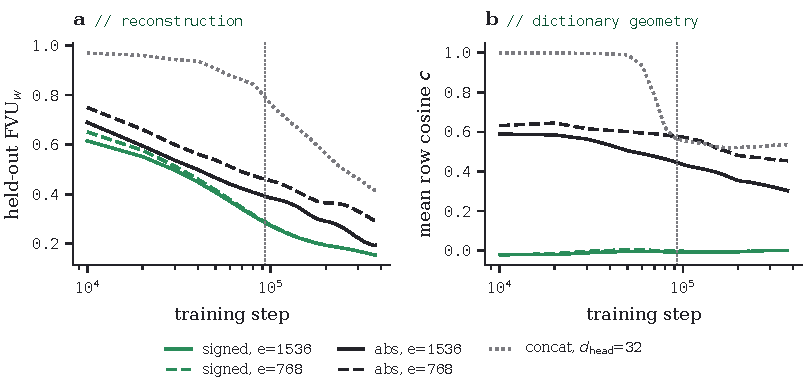
\includegraphics[width=\linewidth]{figures/fig-orthant-curves.pdf}
\caption{The orthant arms over training: held-out $\fvu$ scored from each
checkpoint (a) and mean within-head row cosine (b). The dotted line
marks step 90k. The signed arms coincide at both widths; \texttt{abs} is
behind at both, and further behind at the square decoder.}
\label{fig:orthant-curves}
\end{figure}

Removing the absolute value buys a decorrelated, near-full-rank
dictionary and lower error, roughly what the collinearity setpoint exists
to buy. Signed atoms give up two things: a subtractive feature is harder
to read as ``this concept is present'', and the $\lVert F\rVert_1 \geq h$
floor under \texttt{norm\_rows}, which rests on non-cancellation,
disappears. Concatenated heads, which face a collapsed tradeoff rather
than a raised floor, are the worst arm (Appendix~\ref{sec:concatgeom}).
